% University of Europe for Applied Sciences --- Master's thesis
% Structure and layout follow Prof. Dr. Rand Kouatly, SS 2026
%   "Writing Good thesis" + "Master Colloquium" + "Thesis Structure"
% Compiler: pdfLaTeX   |   Main document: overleaf_main.tex
%
% Fill \Matrikel, \Erstbetreuung, \Zweitbetreuung before binding.
% Confirm any Prüfungsamt wording that differs from the lecture declaration.
\documentclass[12pt,a4paper,oneside]{report}

% UE Master's thesis preamble — Prof. Dr. Rand Kouatly, SS 2026
% Layout from "Writing Good thesis" lecture:
%   margins 2 cm left, 4 cm right, 2.5 cm top, 3 cm bottom
%   Times (Times New Roman equivalent) 12 pt body, 10 pt footnotes
%   justified, 1 cm first-line indent, 6 pt paragraph skip
%   Harvard (author-year) citations
%   DIN 1421 numbering via report class
\usepackage[
  a4paper,
  left=2cm,
  right=4cm,
  top=2.5cm,
  bottom=3cm
]{geometry}
\usepackage[onehalfspacing]{setspace}
\usepackage[T1]{fontenc}
\usepackage[utf8]{inputenc}
\usepackage{mathptmx}
\usepackage{microtype}
\usepackage{booktabs}
\usepackage{tabularx}
\usepackage{array}
\usepackage{enumitem}
\usepackage{graphicx}
\graphicspath{{figures/}{chapters/figures/}}
% Compile even when figure PNGs are not yet exported to Overleaf
\newcommand{\maybeincludegraphics}[2][]{%
  \IfFileExists{#2}{%
    \includegraphics[#1]{#2}%
  }{%
    \fbox{\parbox[c][0.22\textheight][c]{0.92\textwidth}{\centering\small Place \texttt{#2} in the project.}}%
  }%
}
\usepackage{xcolor}
\usepackage{listings}
\usepackage{eurosym}
\usepackage{url}
\usepackage{csquotes}
\usepackage{indentfirst}
\usepackage{tocloft}
\usepackage{caption}
\usepackage{amsmath}
\usepackage{tikz}
\usetikzlibrary{positioning}
\usepackage[round,authoryear,sort]{natbib}
\setcitestyle{authoryear,round,aysep={,},yysep={;}}
\usepackage[hidelinks]{hyperref}

\hypersetup{
  pdftitle={Augmented Analytics on a Production Lakehouse: Integrating Generative AI into European Job Intelligence},
  pdfauthor={Ritesh Rakesh Jadhav}
}

% Paragraph layout (lecture: Justify, 6 Points, Indent 1 cm)
\setlength{\parindent}{1cm}
\setlength{\parskip}{6pt}
\frenchspacing
\raggedbottom

\captionsetup{font=small,labelfont=bf,skip=6pt}
\setlist[itemize]{leftmargin=1.5cm,itemsep=3pt,topsep=4pt}
\setlist[enumerate]{leftmargin=1.5cm,itemsep=3pt,topsep=4pt}

% Harvard paraphrase helper: (cf. Author, Year[, p. x])
\newcommand{\cf}[2][]{\citep[cf.][#1]{#2}}

\lstset{
  basicstyle=\ttfamily\footnotesize,
  breaklines=true,
  frame=single,
  columns=fullflexible,
  keepspaces=true,
  captionpos=b
}

\setcounter{secnumdepth}{3}
\setcounter{tocdepth}{3}


\newcommand{\Matrikel}{[Matriculation number]}
\newcommand{\Erstbetreuung}{[First supervisor --- Prof.\ Dr.\ \ldots]}
\newcommand{\Zweitbetreuung}{[Second supervisor]}
\newcommand{\Abgabedatum}{[Submission date]}
\newcommand{\ThesisTitle}{Augmented Analytics on a Production Lakehouse: Integrating Generative AI into European Job Intelligence}
\newcommand{\ThesisSubtitle}{A Case Study on DataForge}

\begin{document}

% -------------------------------------------------------------------------
% 1. Cover sheet
% -------------------------------------------------------------------------
\begin{titlepage}
\centering
{\large University of Europe for Applied Sciences\par}
\vspace{0.3em}
{\large University of Applied Sciences Europe\par}
\vspace{0.3em}
{\large Faculty of Business / Fachbereich Wirtschaft\par}
\vspace{0.3em}
{\large Campus Potsdam\par}
\vspace{2.2em}
{\LARGE\bfseries \ThesisTitle\par}
\vspace{1em}
{\large \ThesisSubtitle\par}
\vspace{2.2em}
{\large Master's Thesis\par}
\vspace{0.4em}
{\normalsize Programme: M.Sc.\ Data Science\par}
\vspace{1.8em}
\begin{tabular}{rl}
Submitted by: & Ritesh Rakesh Jadhav \\
Matriculation no.: & \Matrikel \\
First supervisor: & \Erstbetreuung \\
Second supervisor: & \Zweitbetreuung \\
Submission date: & \Abgabedatum \\
\end{tabular}
\vspace{1.8em}
\par
Reference implementation: \url{https://github.com/ritesh8303/dataforge}
\vfill
{\small Draft for supervisor review. Print on one side only, on 80\,g/m$^2$ white A4 paper, as required in the writing lecture.}
\end{titlepage}

% -------------------------------------------------------------------------
% Statutory declaration (wording from the SS 2026 writing lecture)
% -------------------------------------------------------------------------
\clearpage
\thispagestyle{empty}
\section*{Statutory Declaration}
\addcontentsline{toc}{chapter}{Statutory Declaration}

\noindent I hereby declare that I have developed and written the enclosed Master Thesis completely by myself and have not used sources or means without declaration in the text. I clearly marked and separately listed all the literature and all the other sources which I employed when producing this academic work, either literally or in content. I am aware that the violation of this regulation will lead to failure of the thesis.

\vspace{2.5em}
\noindent Berlin, \underline{\hspace{6.5cm}}\\[0.4em]
{\small Place, Date}

\vspace{2.5em}
\noindent Signature: \underline{\hspace{7cm}}

\vspace{2em}
\noindent{\small If the Examination Office issues a different official wording, replace this page with that wording before binding.}

% -------------------------------------------------------------------------
% 2. Table of contents
% -------------------------------------------------------------------------
\clearpage
\tableofcontents

% -------------------------------------------------------------------------
% 3. Indices
% -------------------------------------------------------------------------
\clearpage
\chapter*{List of Abbreviations}
\addcontentsline{toc}{chapter}{List of Abbreviations}
\begin{tabular}{@{}ll@{}}
AI    & Artificial Intelligence \\
API   & Application Programming Interface \\
ATS   & Applicant Tracking System \\
AWS   & Amazon Web Services \\
BA    & Bundesagentur f\"ur Arbeit \\
BM25  & Best Match 25 (probabilistic retrieval function) \\
CI    & Continuous Integration \\
DSR   & Design Science Research \\
ECTS  & European Credit Transfer and Accumulation System \\
EU    & European Union \\
GDPR  & General Data Protection Regulation \\
HITL  & Human in the Loop \\
IR    & Information Retrieval \\
LLM   & Large Language Model \\
MCP   & Model Context Protocol \\
MLOps & Machine Learning Operations \\
MRR   & Mean Reciprocal Rank \\
nDCG  & Normalised Discounted Cumulative Gain \\
NLP   & Natural Language Processing \\
RAG   & Retrieval-Augmented Generation \\
RRF   & Reciprocal Rank Fusion \\
RQ    & Research Question \\
SCD   & Slowly Changing Dimension \\
UE    & University of Europe for Applied Sciences \\
\end{tabular}

\clearpage
\listoftables
\addcontentsline{toc}{chapter}{List of Tables}

\clearpage
\listoffigures
\addcontentsline{toc}{chapter}{List of Figures}

% -------------------------------------------------------------------------
% 4. Abstract
% -------------------------------------------------------------------------
\clearpage
\chapter*{Abstract}
\addcontentsline{toc}{chapter}{Abstract}
Job advertisements in Europe are spread across government portals, job websites, and company career pages. DataForge is a live data system on Amazon Web Services (AWS). It already collects job data from several sources and stores it in three layers: Bronze (raw data), Silver (clean history), and Gold (reports). It also offers public Jobs and Metrics APIs. Companies now want more than lists of jobs. They want \emph{augmented analytics}: computer methods that add extra labels to jobs and that match a resume to suitable vacancies. If these AI features are added without tests, they can damage data history, increase cost, and produce results that other people cannot repeat.

This thesis designs, builds, and tests a low-cost generative-AI layer on the existing DataForge system. The layer includes: a model gateway with a stop switch and a budget; rule-based data cleaning first; a language-model path that is \textbf{OpenAI-first} in production while Amazon Bedrock quota stays at zero; hybrid search that combines keyword search (BM25) and meaning-based search (embeddings); a Match API that hides personal data and shows evidence from the job text; and an optional small multi-agent process with a fixed limit. Four research questions study: safe integration (RQ1), model and provider choice (RQ2), matching quality versus the old keyword wizard (RQ3), and cost per job (RQ4).

The study uses design science research with one embedded case. The literature review covers lakehouse design, slowly changing dimensions, information retrieval, LLM operations, and European law. On an expanded labelled test set (103 queries and 96 jobs), meaning-based search reaches the highest nDCG@10 (0.2174) in the packaging run. The old keyword wizard scores 0.1462, and BM25 scores 0.1351. Hybrid retrieval scores 0.1668 on this set. A continuous-integration pin to local tf-idf embeddings later records dense nDCG@10 of 0.1258; that pin is reported as a measurement difference, not as a hidden rewrite of the table. A modelled OpenAI-first path for 1{,}000 jobs (rules first, 30\,\% language-model calls, plus embeddings) is about \EUR{0.10}. Live RQ2 on OpenAI \texttt{gpt-4o-mini} completed 40/40 jobs at about \$0.0011 and 1.1\,s average latency. Amazon Nova Micro remains blocked at zero tokens per minute. Nightly enrichment is on for OpenAI (sample rate 0.25), not for Bedrock.

The thesis argues that generative AI in a production lakehouse must be treated as a controlled pipeline stage. History contracts, non-AI baselines, and honest reporting of missing measurements are as important as model choice.

\vspace{0.8em}
\noindent\textbf{Keywords:} lakehouse; augmented analytics; LLM operations; hybrid search; job matching; cost; responsible AI; European job data.


% -------------------------------------------------------------------------
% 5--11. Numbered chapters (DIN 1421)
% -------------------------------------------------------------------------
\chapter{Introduction}
\label{ch:introduction}

\section{Background and motivation}
\label{sec:motivation}

Job information in Germany and in the European Union is not in one place. It sits on public employment websites, commercial job boards, and company career pages. This is a problem for junior candidates, such as interns, working students, and early-career staff. It is also hard for people who need English-friendly jobs or visa information. Search takes a long time. Job texts mix German and English. Seniority words are not used in the same way. Visa rules are often missing or buried in long descriptions.

The OECD notes that artificial intelligence is changing labour markets. It affects how jobs are advertised, screened, and matched \cf{oecd2023ai}. Public services such as the Bundesagentur f\"ur Arbeit and EURES publish APIs and portals. However, a single candidate still needs to search many channels. Data products that unify public vacancy data can reduce search cost. They must still respect data quality, history, and European law.

DataForge is an applied data-science system that deals with this engineering problem. It already runs as a serverless lakehouse on Amazon Web Services in the Frankfurt region (\texttt{eu-central-1}). It collects data from several sources. It stores raw files in Bronze, historical job versions in Silver, and reports in Gold. It offers public APIs and a GitHub Pages website. This live system is the base of the thesis. The thesis does not start from an empty project.

Industry demand has moved from simple data collection to \emph{augmented analytics}. This means using machine learning and language processing to add labels, find similar jobs, and explain results \cf{provost2013ds,vial2019digital,demiroglu2015dsr}. In software companies, similar ideas appear under names such as hyperautomation and experiment-driven development \cf{fagerholm2017right,gartner2020hyper}. The research problem is not ``build a chatbot''. The problem is: how can generative AI be added to a live pipeline so that data history, repeatable tests, cost, and the law stay under control? Claims must also be possible to test.

\section{Problem statement}
\label{sec:problem}

When companies add large language models to existing data platforms, three problems appear often.

First, \emph{broken data history}. The model may overwrite job IDs or old versions. Then nobody can check what changed. Kimball and Ross warn that slowly changing dimensions need explicit rules. Type~2 history must not be replaced by silent rewrites \cf[p.~~220]{kimball2013dwt}. Second, \emph{quality that is not measured}. Demos show almost perfect ranking scores on tiny examples. They often skip a simple non-AI baseline. IR research has known for decades that ranking must be tested against labels \cf{manning2008ir,jarvelin2002ndcg}. Third, \emph{cost with no limit}. Expensive models are run on all documents. There is no sample rate, no budget, and no stop switch. These problems are part of a wider software issue: hidden extra work in machine-learning systems \cf{sculley2015debt,kreuzberger2023mlops}.

This study uses DataForge as one detailed case. The money limit is small (about \EUR{0}--25 per month in normal use, and a hard thesis cap of \EUR{40}). All cloud work stays in \texttt{eu-central-1}. EU data location is treated as a main design choice, not as a later extra.

\section{Stakeholders and intended use}
\label{sec:stakeholders}

Three stakeholder groups matter for this thesis.

\emph{Job seekers} want shorter lists of relevant vacancies. They care about language, seniority fit, and visa hints. \emph{Platform engineers} want a pipeline that they can operate, pause, and audit. \emph{Supervisors and examiners} want a thesis that connects theory, a built system, and honest evaluation. DataForge Match is designed as \emph{decision support} for seekers. It is not an employer screening tool. This boundary affects both metrics and law, as Chapters~\ref{ch:theory-ai} and~\ref{ch:discussion} explain.

\section{Aim and contribution of the study}
\label{sec:aim}

The aim is to design, build, and test a low-cost generative-AI layer on the existing DataForge lakehouse. The layer has a multi-provider model gateway, rule-based enrichment first, hybrid search for resume--job matching, a Match API that removes personal data, and a repeatable test set.

The thesis has four contributions. First, a reference architecture. Generative models add extra columns. They do not replace job history. Second, a matching experiment. It compares meaning-based search, keyword search, hybrid search, and the old rule-based wizard on a labelled set. Third, a simple cost model. It links model prices and sample rates to product cost. Fourth, a responsible-AI discussion. It maps an advice tool for job seekers to the GDPR and the EU Artificial Intelligence Act \cf{eu2016gdpr,eu2024aiact,veale2021demystifying}.

\section{Link to the Master Colloquium topics}
\label{sec:alignment}

This is an applied Data Science thesis. It is not only a software-engineering paper. It still matches several topics from the Master Colloquium of Prof.\ Dr.\ Rand Kouatly (Summer Semester 2026). The main topics are \emph{augmented analytics} and \emph{hyperautomation}. AI is used to add labels to job text and to automate matching that used to be keyword-based. Secondary topics are \emph{digitalisation of software-intensive services} (what changes when a live data product gets a generative layer) and \emph{automation of data cleaning} (rules first, then expensive language-model calls). Continuous experimentation is the test style: product claims are checked with held-out metrics, not only with a demo story \cf{fagerholm2017right}. Quantum computing, module clustering, and automated fault finding are nearby software topics. They are outside the scope of this thesis.

\section{Structure of the thesis}
\label{sec:structure}

Chapter~\ref{ch:theory-data} reviews digitalisation, lakehouse design, historical data modelling, data quality, and classical information retrieval. Chapter~\ref{ch:theory-ai} reviews language models, dense and hybrid search, retrieval-augmented generation, LLM operations, agents, and EU law. It then states the research gap. Chapter~\ref{ch:rqs} states the research questions and hypotheses. Chapter~\ref{ch:method} explains why design science and a single case study are used. Chapter~\ref{ch:results} reports what was built and what was measured. Chapter~\ref{ch:discussion} discusses the meaning of the results and the limits. Chapter~\ref{ch:implications} discusses theory, practice, and future research.

\section{Scope note for the reader}
\label{sec:scope-note}

The empirical core of this thesis is European public job text and a student-built AWS lakehouse. Results should be read as evidence for frugal GenAI integration under those constraints. They should not be read as a universal ranking of all foundation models, or as a labour-market policy evaluation. Where AWS quota blocked a live Bedrock cell, the text says so. Where labels are author-made, the text says so. That honesty is part of the scientific claim.

\chapter{Theoretical Background I: Data Platforms, Digitalisation, and Information Retrieval}
\label{ch:theory-data}

The literature review is the main academic part of this thesis. It does not list every related paper. It explains the scientific discussion around the DataForge case. It also comments on the quality of the sources. Then it leads to a gap that the later chapters can test. The University of Europe asks students to use sources in a clear order. Peer-reviewed journal papers and conference papers from ACM, IEEE, Springer, Elsevier, and Sage come first. Research books from known publishers are used for basic methods. Official EU laws are primary legal sources. Vendor websites and analyst notes are used only as industry background, and they are marked as such.

\section{Digitalisation and software-intensive labour-market services}
\label{sec:digitalisation}

Digital transformation is often described as a process that tries to improve an organisation by using information, computing, communication, and network technologies together \cf[p.~~118]{vial2019digital}. Digitisation of a PDF is only a small step. Digitalisation of a job service means that software is the main way jobs are published, found, ranked, and explained. Fitzgerald and colleagues argued that using digital technology is now a core business need, not an optional IT project \cf{fitzgerald2014digital}. For public employment services and job platforms, this is visible in APIs from the Bundesagentur f\"ur Arbeit and from EURES, and in many applicant-tracking systems in companies \cf{ba2024jobsuche,eures2024}.

Two points matter for data science. First, job data is not a single static file. It comes from many sources, and the field names do not always match. Second, matching and enrichment are software products. Quality attributes from software architecture still apply: change is possible, the service is available, cost is controlled, and security is kept \cf{bass2012architecture,iso25010}. The colloquium theme ``digitalisation and digital transformations: impacts on software engineering'' is therefore a real condition of this work. A lakehouse and a generative-AI layer must work together.

Labour-market research also warns that AI can change hiring and job search at scale \cf{oecd2023ai,webb2020double}. This thesis does not predict macro employment effects. It treats job intelligence as a \emph{software service} whose quality can be measured on retrieval metrics and operational limits.

\section{From warehouses to lakehouses}
\label{sec:lakehouse}

For a long time, enterprise analytics used two main ideas. Bill Inmon described a central, normalised data warehouse. Ralph Kimball described dimensional models that are easier for reports \cf{inmon2005bdw,kimball2013dwt}. Both ideas assume that a clean database is the main source for decisions. Later, ``data lakes'' stored cheap files first and added structure later. Armbrust and co-authors argue that neither extreme is enough. A \emph{lakehouse} tries to keep warehouse controls (transactions, schema, governance) and also keep the scale of lakes \cf{armbrust2021lakehouse}.

In industry, this is often built as a medallion pattern: Bronze for raw ingest, Silver for cleaned history, and Gold for user reports \cf{databricks2020medallion}. The word ``medallion'' is not a peer-reviewed theory by itself. It is a common engineering pattern. It can be criticised and tested. The stronger scientific ideas are older: improve data step by step, keep raw evidence separate from later metrics, and write clear contracts between layers. These ideas later limit how generative outputs may enter the pipeline.

For DataForge, the lakehouse is not an abstract diagram. Bronze keeps raw Parquet from each source. Silver owns job identity and history. Gold joins aggregates and API-facing tables. Any generative enrichment must respect these contracts. Otherwise the system repeats the technical debt that Sculley and colleagues describe for machine-learning systems glued onto legacy pipelines \cf{sculley2015debt}.

\section{Historical modelling and slowly changing dimensions}
\label{sec:scd}

Job postings change. Titles are rewritten. Locations appear and disappear. Vacancies close. Kimball and Ross call such entities slowly changing dimensions. Type~1 overwrites the old value. Type~2 keeps history by adding a new row with start and end dates \cf[p.~~193]{kimball2013dwt}. For labour-market analytics, Type~2 is important. Without it, we cannot answer time questions, such as how long internships stay open, or how visa wording changes. A language model that silently rewrites the current row would destroy this history.

This thesis therefore uses a strict rule. Generative enrichment may \emph{join} Silver and Gold. It must not change business keys or slowly changing dimension date fields. This is an application of dimensional modelling to a modern machine-learning setting. It is not a new modelling theory.

\section{Data quality and the automation of cleaning}
\label{sec:quality}

Poor data quality has long created hidden costs for organisations \cf{redman1998dq}. Batini and colleagues review methods to assess and improve quality. They use dimensions such as accuracy, completeness, consistency, and timeliness \cf{batini2009dq}. Demirkan and Delen link information quality to measurable profiles that can guide improvement work \cf{demiliani2006dq}. In modern analytics, cleaning is not a one-time script. It is ongoing software work. This is why the colloquium lists ``automation of data cleaning'' as a data-science topic.

Two implications matter here. First, clear rules (regular expressions, taxonomies, schema checks) are still strong quality tools. They are cheaper, easier to inspect, and easier to repeat. Second, language models can help when rules are unclear. However, they can also produce fluent labels that are not grounded in the text. A careful architecture therefore applies rules first. It spends model tokens only on the remaining unclear cases. This idea returns as a cost hypothesis in Chapter~\ref{ch:rqs}.

In job text, quality problems are domain-specific. Seniority may appear as ``Werkstudent'', ``Praktikum'', ``Junior'', or ``(m/w/d)'' with no level at all. Visa stance may be explicit, implied, or absent. Language requirements may be split between title and body. Rules can catch many patterns in German and English. They cannot catch every employer style. That mixed picture motivates a \emph{rules-first, model-second} enrichment design.

\section{Classical information retrieval}
\label{sec:classical-ir}

Matching a resume to a job is, at root, an information-retrieval (IR) problem. A query (the candidate profile) is ranked against a collection of job documents. Manning, Raghavan and Sch\"utze give a standard textbook for this field. They cover Boolean search, ranked search, evaluation, and web search \cf{manning2008ir}. Among keyword rankers, BM25 is still the main probabilistic baseline. Robertson and Zaragoza present BM25 in the probabilistic relevance framework. They explain why term-frequency limits and document-length normalisation often beat simple tf--idf \cf{robertson2009bm25}.

Keyword methods fail in known ways on job text. A candidate who writes ``PyTorch'' will not match a posting that only says ``deep learning framework''. Mixing German and English makes this worse. A query for ``Werkstudent'' may miss a posting titled ``Working Student'' if tokenisation is naive. These failures motivate meaning-based (dense) retrieval, which is reviewed in the next chapter. They also explain why a keyword Career Matching Wizard is a fair scientific baseline. It is clear, cheap, and similar to many live systems.

\section{Evaluation of ranked retrieval}
\label{sec:ir-eval}

IR research says that ranking quality must be measured against relevance labels, not against user stories only. Precision at $k$, recall at $k$, and mean reciprocal rank are standard metrics \cf[p.~~159]{manning2008ir}. For graded relevance, J\"arvelin and Kek\"al\"ainen introduced discounted cumulative gain and its normalised form nDCG. nDCG gives more reward when highly relevant documents appear near the top, and it can be compared across queries \cf{jarvelin2002ndcg}. This thesis uses nDCG@10 as the main matching metric. Precision@5, Recall@20, and MRR are extra measures.

Two warnings from IR research limit later interpretation. First, a small labelled set supports an applied master's pilot. It does not support a very large IR benchmark claim. Second, if the person who writes labels thinks in synonyms, dense methods may look better than they are. A simple keyword baseline is therefore a needed control. It is not a weak joke comparison.

Benchmark work such as BEIR shows that retrieval models behave very differently across domains \cf{thakur2021beir}. A model that wins on news may lose on biomedical text. Job text in Europe is another domain. It mixes languages, HR boilerplate, and sparse structured fields. This thesis does not claim BEIR-scale evidence. It does claim that domain-specific labels are necessary.

\section{Person--job matching as a special retrieval task}
\label{sec:jobmatch}

Recommending jobs to people, and people to jobs, is a two-sided matching problem \cf{malinowski2006matching}. Neural person--job fit models later represent skills and job requirements in a shared space \cf{qin2018personjob}. Surveys of deep learning for job recommendation list challenges such as short text, skill mismatch, and cold-start vacancies \cf{guo2019deep,rahmani2022jobrec}. Industry systems also face fairness issues. Work on LinkedIn talent search shows that exposure can be unbalanced, and that fair re-ranking is an active topic \cf{geyik2019fairness}.

For an advice system aimed at job seekers, two differences are important. The system ranks \emph{public vacancies} for a user who gave a resume. It does not rank \emph{candidates} for a hiring manager. This difference later supports the legal discussion. It also explains why this study uses IR metrics on job rankings, and not hiring-outcome metrics that cannot be observed here.

Barocas, Hardt and Narayanan stress that fairness depends on the decision context and on what is measured \cf{barocas2023fairness}. A seeker-side ranker can still harm users if it hides viable jobs or over-promotes others. Holstein and colleagues report that practitioners need concrete tooling and process support, not only abstract fairness definitions \cf{holstein2019improving}. These points motivate citations, human review for low confidence, and honest limits in product copy.

\section{Multi-source ingest and public employment data}
\label{sec:multisource}

European job intelligence must combine heterogeneous sources. Public APIs from the Bundesagentur and EURES provide official listings \cf{ba2024jobsuche,eures2024}. Commercial boards and company ATS feeds add coverage. Each source uses different field names, update frequencies, and language habits. Inmon's warehouse idea of a single integrated store still applies, but the integration work is continuous \cf{inmon2005bdw}.

From a research view, multi-source ingest raises three quality questions. \emph{Coverage:} does the corpus include the roles the queries ask for? \emph{Freshness:} are closed jobs removed quickly? \emph{Provenance:} can a match cite the job ID and source? DataForge keeps source tags and job IDs stable through Silver. Match results expose \texttt{job\_id} and evidence spans. These choices follow IR and software-architecture practice more than a new theory.

\section{Continuous experimentation as a test style}
\label{sec:experimentation}

Software product teams more often test development decisions with experiments, not only with expert opinion. Fagerholm and colleagues present the RIGHT model for continuous experimentation. They argue that experiment-driven development reduces the risk of building the wrong product \cf{fagerholm2017right}. This thesis does not run a long online A/B test with live job seekers. The time of a master's project is short. It is also not ethical to put untested rankers into a public user interface. The thesis still uses the experiment idea: every generative claim has a protocol, a baseline, and a metric. This is how the colloquium topic ``continuous experimentation'' is used.

\section{Literature map and critique}
\label{sec:lit-critique}

Table~\ref{tab:lit-map} maps literature streams to what they contribute, and to what they usually omit in practitioner writing.

\begin{table}[ht]
\centering
\caption{Literature streams and their limits for this case}
\label{tab:lit-map}
\begin{tabularx}{\textwidth}{@{}lXX@{}}
\toprule
\textbf{Stream} & \textbf{Main contribution} & \textbf{Typical gap for DataForge} \\
\midrule
Digitalisation & Explains why job services are software products & Rarely gives pipeline contracts \\
Lakehouse / medallion & Layered storage and governance & Rarely treats generative outputs as SCD-safe joins \\
Data quality & Rules and measurement dimensions & Rarely combines with token budgets \\
Classical IR & Baselines and nDCG & Rarely uses junior/visa query mixes \\
Person--job fit & Neural matching ideas & Often employer-side; weak on EU law \\
MLOps & Versioning and monitoring & Weak on FrugalGPT-style routing at small budget \\
\bottomrule
\end{tabularx}
\end{table}

Several sources in Table~\ref{tab:lit-map} are strong but not perfect. Armbrust et al.\ describe lakehouses at platform level; they do not discuss GDPR resume handling \cf{armbrust2021lakehouse}. Geyik et al.\ study employer-side fairness; this thesis studies seeker-side ranking \cf{geyik2019fairness}. Rahmani and Bhulai review recommenders; many listed papers target English-only corpora \cf{rahmani2022jobrec}. These limits are normal in a focused master's review. They also define where this thesis adds value: integration under European production limits.

\section{Interim summary}
\label{sec:interim1}

The first theory chapter leads to five points. Digitalisation makes labour-market software a data-science object, not only a scraping task. Lakehouse and medallion patterns give layer contracts. Slowly changing dimensions forbid silent rewrites of history. Data-quality research supports rules before tokens. Classical IR and person--job matching research give metrics and a non-AI baseline. The next chapter studies what generative models change, and what they must not be allowed to change.

\section{Positioning against pure software portfolios}
\label{sec:portfolio-gap}

Many student portfolios show scrapers or dashboards without a held-out ranking test. Many applied AI demos show a chat box without lineage or cost logs. The gap that this thesis fills is the combination of both sides: a live medallion system with SCD Type~2 history, and a GenAI layer that is measured against a transparent non-AI baseline. Related work on lakehouses explains storage and refinement \citep{armbrust2021lakehouse}. Related work on dense retrieval explains ranking quality \citep{karpukhin2020dpr,jarvelin2002ndcg}. Related work on LLMOps explains operations \citep{kreuzberger2023mlops}. Few single sources require all three in one applied master's artefact. That is why the literature chapters stay long even though the artefact is software-intensive.


\chapter{Theoretical Background II: Generative AI, Retrieval Systems, and Responsible Automation}
\label{ch:theory-ai}

\section{Transformer language models}
\label{sec:transformers}

Today's generative models are based on the transformer architecture. Transformers use self-attention instead of older recurrent networks. This makes large-scale pre-training more practical \cf{vaswani2017attention}. Encoder models such as BERT showed that pre-trained text representations transfer well to search and classification after fine-tuning \cf{devlin2019bert}. Very large decoder models, such as GPT-3, showed that a model can solve new tasks from examples in the prompt, without changing weights \cf{brown2020gpt3}. Jurafsky and Martin give a textbook view of how tokenisation, embeddings, and sequence models fit together in modern NLP pipelines \cf{jurafsky2023speech}.

Foundation-model reports later argued that a small number of large models may become shared infrastructure. They also warned about opacity and concentration of power \cf{bommasani2021foundation}. For this thesis, the practical lesson is simple. Encoder-style embeddings are the right tool for meaning-based matching. Decoder-style completion models are the right tool for writing extra labels and explanations. Mixing the two without a plan increases cost. There is no need to generate a paragraph only to rank a document. Chain-of-thought prompting can help reasoning on some tasks \cf{wei2022cot}, but it also uses more tokens. A low-cost design therefore treats generation as an expensive, optional step.

\section{Dense retrieval, embeddings, and retrieval-augmented generation}
\label{sec:dense}

Dense passage retrieval turns queries and documents into vectors in the same space. It then finds nearest neighbours. On several open-domain question-answering tests, it beat BM25 \cf{karpukhin2020dpr}. Sentence-BERT showed that a special training setup produces embeddings that work well for clustering and semantic search. Simple BERT CLS vectors often do not \cf{reimers2019sbert}. Lin, Nogueira and Yates review later work on transformers for ranking. Cross-encoders can be more accurate, but they are expensive on a large collection \cf[p.~~45]{lin2021transformers}. Gao et al.\ discuss zero-shot dense retrieval when no in-domain labels exist \cf{gao2023precise}. That setting is close to a cold-start job corpus, although this thesis \emph{does} use a small labelled set for evaluation.

Retrieval-augmented generation (RAG) joins a retriever (the documents) with a generator (the language model). This can reduce invented facts on knowledge-heavy tasks, compared with generation only \cf{lewis2020rag}. Recent surveys list open problems: citation faithfulness, latency, and evaluation of grounded answers \cf{wang2024rag}. In a job-matching product the same idea is: first retrieve a short list of vacancies with embeddings, then optionally ask a language model to explain or re-rank that short list, with citations. The generator must not invent jobs. This is both an IR design pattern and a responsible-AI control.

\section{Hybrid retrieval and rank fusion}
\label{sec:hybrid}

Keyword rankers and dense rankers fail on different queries. Hybrid pipelines therefore combine BM25 with dense scores. Reciprocal rank fusion (RRF) is a simple method for merging ranked lists. Cormack, Clarke and Buettcher showed that RRF can beat more complex learning-to-rank combinations on several collections \cf{cormack2009rrf}. Thakur et al.\ show on BEIR that no single retriever wins on all dataset types \cf{thakur2021beir}. Hybrid retrieval is therefore the usual engineering default in many production RAG stacks, even when one labelled set favours pure dense retrieval.

This difference between \emph{best score on one gold set} and \emph{best default for a product with several goals} will later explain a design choice. DataForge may still use hybrid matching even if dense retrieval has a higher nDCG@10. A thesis that reports only the winning number would be incomplete. A thesis that reports the number and the reasons for not using it blindly is closer to applied data science.

\section{Augmented analytics and hyperautomation}
\label{sec:augmented}

Augmented analytics means using machine learning and natural language processing to automate parts of data preparation, insight, and explanation that used to need a specialist \cf{provost2013ds}. Hyperautomation, a term used by industry analysts, goes further. It says that if a business process can be automated, it should be automated, by combining analytics, process tools, and robots \cf{gartner2020hyper}. Both terms sit next to the colloquium topic list. They are also easy to over-claim.

A careful academic use of these terms needs three limits. First, automation is a means, not the goal. ISO/IEC 25010 quality characteristics still apply to the system \cf{iso25010}. Second, not every step should go to a large language model. Rules, indexes, and tests are also automation. They are cheaper and easier to audit. Third, ``real-time insight'' is a claim about speed and freshness. It is not the same as ``we called an API''. The architecture in this thesis is therefore a \emph{limited} case of augmented analytics. Enrichment and matching are automated under budgets. The lakehouse contracts stay human-defined.

\section{MLOps, LLMOps, and cost--quality routing}
\label{sec:llmops}

Sculley and colleagues warned that machine-learning systems collect hidden technical debt. Causes include tight coupling, extra users that were not planned, and glue code \cf{sculley2015debt}. MLOps literature answers with life-cycle practices: versioning, monitoring, continuous delivery, and governance of models as software \cf{kreuzberger2023mlops}. Empirical lists of software-engineering challenges for machine learning also stress data management, experiment tracking, and the gap between research and production \cf{lwakatare2019mlse}. Raji et al.\ propose internal algorithmic auditing as a way to close accountability gaps before deployment \cf{raji2020closing}.

Large language models add a billing problem that older MLOps work did not stress enough. Chen, Zaharia and Zou show that sending easy cases to cheap models and hard cases to expensive models (FrugalGPT) can match the quality of one strong model at much lower cost \cf{chen2023frugalgpt}. For a master's system with a free-tier budget, the lesson is direct. A task-aware router with daily budgets is part of the research design. It is not only an extra feature. Multi-provider routing also encodes an EU choice: inference in the region (for example Amazon Bedrock in Frankfurt) versus US software-as-a-service APIs. Quality, cost, latency, and data location are therefore several goals at once. They are not a single accuracy table.

\section{Agents and tool use}
\label{sec:agents}

Tool-using agents mix reasoning steps with actions, as in the ReAct pattern \cf{yao2023react}. A graph of specialist steps can, in principle, split retrieval, scoring, explanation, and checking. The scientific warning is clear. Open-ended agent loops are hard to cost, hard to test, and hard to explain when they fail. This thesis therefore treats agents as an optional, \emph{limited} graph. There is a fixed maximum number of language-model calls and handoffs. The Model Context Protocol bridge is a thin tool interface. It is not an independent workforce. This limit matches the low-cost stance of the previous section.

\section{Responsible AI, GDPR, and the EU Artificial Intelligence Act}
\label{sec:responsible}

Algorithm systems raise ethics issues of opacity, bias, and accountability. These issues existed before generative models \cf{mittelstadt2016ethics}. Frameworks such as AI4People turn those issues into principles: do good, avoid harm, respect autonomy, be fair, and be able to explain \cf{floridi2018ai4people}. Jobin, Ienca and Vayena map hundreds of AI ethics guidelines globally. They show convergence on transparency and accountability, but weak operational detail \cf{jobin2019global}. In European law, two instruments dominate.

The General Data Protection Regulation requires lawful, fair, and transparent processing. It also requires purpose limitation, data minimisation, and storage limitation for personal data \cf{eu2016gdpr}. A matching service that accepts a resume processes personal data, even if job text is public. Removing personal data, using the resume only for job discovery, and avoiding extra profiling are therefore design requirements. They are not only an ethics appendix. Veale et al.\ discuss how model inversion and memorisation create legal risk even when outputs look anonymised \cf{veale2018fairness}.

The Artificial Intelligence Act uses a risk-based system \cf{eu2024aiact}. Some AI systems used in employment and access to work are high-risk when they are used to recruit or to decide about an employment relationship. Veale and Borgesius explain the draft and final structure for practitioners \cf{veale2021demystifying}. An advice ranker of \emph{public vacancies} for a job seeker is a different use from an employer tool that ranks \emph{people}. Mixing these two uses would over-state legal risk in one way, and under-state remaining duties of transparency and human oversight in another way. Wachter, Mittelstadt and Floridi have also argued that a general ``right to explanation'' of automated decisions is weaker in the GDPR than popular comments suggest \cf{wachter2017explanation}. Edwards and Veale discuss how users may still deserve \emph{better decisions} and meaningful information even when a full explanation right is narrow \cf{edwards2021regulating}. Product-level citations and disclaimers are therefore an ethics design choice, and they may also reduce legal risk.

Selbst et al.\ warn that fairness discussions often abstract away the sociotechnical system \cf{selbst2019fairness}. For DataForge, the sociotechnical picture includes: public job text, a user-uploaded resume, a GitHub Pages wizard, and optional API keys. Responsible design must fit that whole path, not only the embedding model.

\section{Design science as the frame for building a system}
\label{sec:dsr-theory}

Information-systems research separates behavioural science, which explains phenomena, from design science, which builds and evaluates artefacts to solve identified problems \cf[p.~~75]{hevner2004dsr}. Peffers and colleagues describe a process: identify the problem, set objectives, design and develop, demonstrate, evaluate, and communicate \cf{peffers2007dsr}. Vom Brocke and Maedche later offer a planning grid for such projects \cf{vomBrocke2015dsr}. Gregor and Hevner explain how to position design science so that contributions are visible to reviewers \cf{gregor2013positioning}. Gregor also classifies types of theory in information systems. This thesis mainly produces an \emph{analytical} and \emph{explanatory} contribution about integration, not a new grand law \cf{gregor2007theory}.

Design science is the right frame because this thesis produces a working system (the integration layer), not only a statistical model. It is not a licence to skip theory. Hevner requires that artefacts rest on existing theories and that evaluation methods match the claims. The base theories here are dimensional modelling, IR evaluation, MLOps, and European data-protection law. The evaluation methods are a labelled ranking experiment, a cost model, and an architecture argument about data history. Yin's case-study logic supports design science. It justifies one current, information-rich case---DataForge---when the questions are of the ``how'' and ``why'' type \cf{yin2018casestudy}.

\section{Research gap}
\label{sec:gap}

Each reviewed stream is mature on its own. Lakehouses, SCD Type~2, BM25, dense retrieval, RAG, MLOps, and the AI Act are not forgotten topics. What is still thin in applied master's work and in practitioner writing is their \emph{joint} use under production limits:

\begin{enumerate}
  \item a live multi-source medallion system with history contracts that must not be broken;
  \item a generative layer with stop switches, budgets, and EU location limits;
  \item a matching experiment that can fail, and that keeps an honest non-AI baseline;
  \item a cost discussion based on token prices and sample rates, not on slide return-on-investment.
\end{enumerate}

New chatbot studies usually skip (1). Pure data-engineering theses usually skip (2)--(4). Vendor white papers usually skip (3). The gap of this thesis is therefore an integration gap. It is not a claim that embeddings or lakehouses are new.

\section{Interim summary}
\label{sec:interim2}

Generative models change how matching and enrichment can be built. They do not cancel IR evaluation, dimensional history, or European law. Augmented analytics is used here as limited automation of enrichment and retrieval. LLM operations and FrugalGPT-style routing supply the cost discipline. Design science plus a single-case study supply the research method that Chapter~\ref{ch:method} will defend. The research questions in the next chapter turn the gap into empirical work.

\section{Summary of the theory chapters}
\label{sec:theory-summary}

Chapter~2 and this chapter together give the theoretical background that the colloquium structure requires. Lakehouse and SCD Type~2 theory explain why GenAI must not rewrite identity keys. Retrieval theory explains why nDCG@10 and a non-AI baseline are used. LLMOps and FrugalGPT explain budgets and routers. GDPR and the AI Act explain why seeker-side ranking is treated as advisory search rather than employer selection. Design science explains why building and evaluating one artefact is a valid master's method. The next chapters state the research questions and the concrete method used on DataForge.

\chapter{Research Questions}
\label{ch:rqs}

\section{Objectives}
\label{sec:objectives}

The general objective is to find out how generative AI can be added to an existing European job-data lakehouse. Data history, honest evaluation, cost control, and legal duties must stay intact. The specific objectives are:

\begin{enumerate}
  \item to write layer contracts so that enrichment and matching only add data to Silver and Gold;
  \item to build a multi-provider gateway with task types, logs, and a stop switch;
  \item to compare keyword, dense, hybrid, and rule-based matching on a labelled query set;
  \item to estimate the cost of rules-first enrichment and embeddings for 1{,}000 jobs;
  \item to map the system to GDPR and AI Act duties for an advice tool for job seekers.
\end{enumerate}

\section{Research questions}
\label{sec:questions}

Table~\ref{tab:rqs} states the four research questions. They are mixed on purpose. RQ1 is about architecture. RQ2 and RQ3 are empirical. RQ4 is about cost. This mix matches a design-science thesis, which must both build a system and evaluate it \cf{hevner2004dsr}.

\begin{table}[ht]
\centering
\caption{Research questions}
\label{tab:rqs}
\begin{tabularx}{\textwidth}{@{}lX@{}}
\toprule
\textbf{ID} & \textbf{Question} \\
\midrule
RQ1 & How can generative AI be added to an existing Bronze$\rightarrow$Silver$\rightarrow$Gold$\rightarrow$API lakehouse without breaking SCD Type~2 history, repeatable tests, or a low-budget cost limit? \\
RQ2 & For enrichment and related tasks, which provider or model class is best on quality, cost, latency, and EU data location? \\
RQ3 & Do embeddings and hybrid retrieval beat the existing 60/20/20 rule-based Career Matching Wizard on ranked job relevance? \\
RQ4 & Under which product packaging does AI-on-pipeline give better unit cost than selling raw open job files only? \\
\bottomrule
\end{tabularx}
\end{table}

\section{Hypotheses}
\label{sec:hypotheses}

The testable hypotheses for RQ2--RQ4 are:

\begin{itemize}
  \item \textbf{H1.} Dense or hybrid retrieval improves nDCG@10 compared with the rule-based wizard on a held-out labelled query set.
  \item \textbf{H2.} Cheap or small models, used only when rules are unclear, are enough for structured enrichment in this domain, compared with unlimited frontier models.
  \item \textbf{H3.} A task-aware router with budgets reduces spend at similar quality, compared with always using one unconstrained provider.
  \item \textbf{H4.} Match and enrichment features give better euro-per-value economics than selling raw CSV extracts of public jobs alone.
\end{itemize}

RQ1 is evaluated with architecture contracts and operational evidence (keys that cannot change, extra columns only, stop switch, budget runbook). It is not evaluated with one single score.

\section{Scope and limits of the questions}
\label{sec:rq-scope}

The questions are about \emph{integration} of generative models into one live case. They are not about inventing a new retrieval algorithm. They do not ask whether language models can replace public employment services. They also do not ask whether an employer ranking system is fair. Visa-related fields are advice signals extracted from text. They are not legal advice. Live multi-provider tests for RQ2 depend on cloud-account quotas. If quotas block measurement, the thesis reports a fixed test method. It does not invent a result table.

\chapter{Methodology}
\label{ch:method}

\section{Choice of research methodology}
\label{sec:method-choice}

A master's thesis must not only use a method. It must also explain why this method is used, and why other methods are not used \cf[p.~~3]{bryman2012social}. Three options were considered: a literature review without a built system; a survey of practitioners; and a design-science study with one embedded case.

\subsection{Why not literature review only?}

A literature-only thesis can summarise the current scientific discussion. The University of Europe treats this as an important academic skill. However, it cannot answer RQ1--RQ4. Those questions ask how integration behaves under cost, data history, and ranking metrics. Hevner argues that design science must produce and evaluate artefacts when the problem is practical and contextual \cf{hevner2004dsr}. Reading about lakehouses and RAG is not enough to show that SCD keys stay unchanged in \emph{this} Terraform stack.

\subsection{Why not a survey?}

A survey of data engineers or career-platform owners could measure beliefs about augmented analytics. Surveys are strong when the research question is about opinions, prevalence, or attitudes \cf{bryman2012social}. They are weak when the question needs reproducible ranking scores, token-cost logs, and code inspection. Holstein et al.\ show that practitioner needs for fair ML systems are often vague until a concrete tool exists \cf{holstein2019improving}. In this thesis, the concrete tool \emph{is} the object of study. A survey would also add ethics workload (sampling, consent, anonymity) without replacing the need for labelled retrieval tests.

\subsection{Why not a laboratory-only experiment?}

A controlled experiment on synthetic job text could isolate one retrieval algorithm. That design improves internal validity for a single metric. It drops the production limits that form the gap in Chapter~\ref{ch:theory-ai}: multi-source ingest, SCD history, EU region routing, quota pauses, and a rule-based wizard baseline that already runs in production. Yin notes that case studies are justified when the researcher asks \emph{how} and \emph{why} in a real context \cf[p.~~15]{yin2018casestudy}. The generative layer is such a context.

\subsection{Chosen design: design science with an embedded case}

The chosen design is therefore \textbf{design science research} in the sense of Hevner and of Peffers. DataForge is an \textbf{embedded single-case study} in the sense of Yin \cf{hevner2004dsr,peffers2007dsr,yin2018casestudy}. The artefact is the generative integration layer. The case gives the live lakehouse, the rule-based baseline, and the money limit. Evaluation combines a labelled IR experiment, a cost model, and an architecture check. Gregor and Hevner recommend stating the artefact type, the contribution, and the evaluation method clearly \cf{gregor2013positioning}. Table~\ref{tab:dsr-mapping} maps Peffers's process steps to this thesis.

\begin{table}[ht]
\centering
\caption{Design science process mapped to thesis activities}
\label{tab:dsr-mapping}
\begin{tabularx}{\textwidth}{@{}lX@{}}
\toprule
\textbf{Peffers step} & \textbf{This thesis} \\
\midrule
Problem identification & Broken history, unmeasured quality, unbounded LLM cost (Chapter~\ref{ch:introduction}) \\
Objectives & RQ1--RQ4 and requirements tables below \\
Design \& development & Gateway, rules-first enrichment, hybrid Match API, eval harness \\
Demonstration & Deployment on AWS \texttt{eu-central-1} lakehouse \\
Evaluation & nDCG experiment, ROI model, architecture audit, ablation \\
Communication & Thesis, repository, colloquium \\
\bottomrule
\end{tabularx}
\end{table}

\section{Advantages and disadvantages of the chosen design}
\label{sec:method-tradeoffs}

The advantages are clear. We can check whether SCD keys stay unchanged. The pipeline is real. The design also matches an applied M.Sc.\ Data Science profile. The disadvantages are also clear. One case does not statistically generalise to all lakehouses \cf{yin2018casestudy}. Labels written by the author can favour dense methods. Cloud quotas can block parts of the measurement plan. These disadvantages are treated as threats to validity in Chapter~\ref{ch:results}. They are not surprises.

\section{Research process}
\label{sec:process}

Following Peffers et al., the process has six steps.

\begin{enumerate}
  \item \textbf{Problem identification.} Broken data history, quality that is not measured, and cost with no limit on live pipelines (Chapter~\ref{ch:introduction}).
  \item \textbf{Objectives of a solution.} Extra columns only, measurable matching, routing that respects EU location, and unit cost (Chapter~\ref{ch:rqs}).
  \item \textbf{Design and development.} Gateway, rules-first enrichment, hybrid retrieval, Match API, evaluation harness.
  \item \textbf{Demonstration.} Deployment on the existing AWS lakehouse in \texttt{eu-central-1}.
  \item \textbf{Evaluation.} RQ1--RQ4 protocols below.
  \item \textbf{Communication.} This thesis, the repository, and the Master Colloquium presentation.
\end{enumerate}

\section{The existing system as empirical context}
\label{sec:context}

Before the generative layer, DataForge already provided the components in Table~\ref{tab:baseline}. Region and infrastructure-as-code (Terraform, S3 state) are part of the case. They limit data location and cost.

\begin{table}[ht]
\centering
\caption{Baseline DataForge components used as case context}
\label{tab:baseline}
\begin{tabularx}{\textwidth}{@{}lX@{}}
\toprule
\textbf{Component} & \textbf{Role} \\
\midrule
Ingest Lambdas and GitHub Actions & Arbeitnow, BA, ATS/Personio, Berlin startups, EURES, later Himalayas/HN \\
Bronze on S3 & Raw Parquet, short retention \\
Silver on S3 & SCD Type~2 job history \\
Gold on S3 plus aggregates & Analytics CSVs, metrics, dbt/DuckDB path \\
API Gateway & Jobs search and metrics \\
GitHub Pages & Dashboard, job board, rule-based Career Matching Wizard \\
\bottomrule
\end{tabularx}
\end{table}

The layer contracts for RQ1 cannot be broken. Bronze must not invent business KPIs. Silver owns identity and SCD validity. Gold may use extra enrichment joins. Quality gates (Pydantic ingest, region taxonomy, CI, dbt tests) stay in control.

\section{Artefact requirements}
\label{sec:requirements}

Functional requirements of the integration layer are shown in Table~\ref{tab:func-req}. Non-functional requirements are shown in Table~\ref{tab:nfr}.

\begin{table}[ht]
\centering
\caption{Functional requirements of the generative integration layer}
\label{tab:func-req}
\begin{tabularx}{\textwidth}{@{}lX@{}}
\toprule
\textbf{ID} & \textbf{Requirement} \\
\midrule
F1 & Rules-first German/English classification for field, seniority, visa stance, and languages \\
F2 & Optional language-model enrichment only when rules are unclear or a sample rate allows it \\
F3 & Hybrid BM25 plus dense retrieval with reciprocal rank fusion; optional LanceDB-on-S3 \\
F4 & Match API with citations that include \texttt{job\_id} and evidence spans \\
F5 & Personal-data removal before language-model calls; API key on production Match \\
F6 & Optional limited multi-agent graph and human-in-the-loop queue for low confidence \\
F7 & Model Context Protocol tools over HTTPS Match/Jobs \\
F8 & Evaluation harness and continuous-integration gates against almost-perfect scores \\
\bottomrule
\end{tabularx}
\end{table}

\begin{table}[ht]
\centering
\caption{Non-functional requirements}
\label{tab:nfr}
\begin{tabularx}{\textwidth}{@{}lX@{}}
\toprule
\textbf{ID} & \textbf{Requirement} \\
\midrule
N1 & Hard cost limit (\EUR{40} thesis cap; daily budget on the router) \\
N2 & Stop switch \texttt{AI\_ENABLED} \\
N3 & Prefer EU-resident inference (Bedrock in \texttt{eu-central-1}) when quota allows; OpenAI-first in production while Nova Micro quota is 0 \\
N4 & Repeatable test files under \texttt{evals/} \\
N5 & Honest claims: no ``live AI'' wording when a quota pause applies \\
\bottomrule
\end{tabularx}
\end{table}

\section{Evaluation protocols}
\label{sec:eval-protocol}

Table~\ref{tab:method} maps experiments to research questions. Matching uses 103 graded queries against 96 jobs (expanded from a 42-query pilot). nDCG follows J\"arvelin and Kek\"al\"ainen \cf{jarvelin2002ndcg}. The rule-based wizard (60\,\% skills, 20\,\% seniority, 20\,\% location) is the non-AI baseline required by H1.

\begin{table}[ht]
\centering
\caption{Evaluation protocols}
\label{tab:method}
\begin{tabularx}{\textwidth}{@{}lXX@{}}
\toprule
\textbf{Experiment} & \textbf{Protocol} & \textbf{Metric} \\
\midrule
Matching (RQ3) & 103 $\times$ 96; BM25, dense, hybrid, heuristic & nDCG@10, P@5, Recall@20, MRR \\
Rules enrichment & 150 labelled jobs; field, seniority, visa & Precision, recall, F1 \\
Agent ablation & 30 queries; hybrid versus multi-agent & Citation-structure validity \\
Faithfulness spot-check & 20 hybrid citations (offline fixture) & Structural validity; optional LLM judge \\
RQ2 Pareto & Rules versus pinned OpenAI \texttt{gpt-4o-mini} (n=40); Bedrock if quota allows & Latency, euro cost, success rate \\
ROI model (RQ4) & Public prices $\times$ token scenario + live CostLogger & Euro per 1{,}000 jobs \\
\bottomrule
\end{tabularx}
\end{table}

\subsection{Construct validity}

Construct validity asks whether metrics measure the intended concept \cf{bryman2012social}. nDCG@10 measures ranked relevance on author labels. It does not measure hiring success, salary, or user satisfaction. That limit is accepted. The construct is ``useful ordering of public vacancies for a stated profile'', not ``employer choice''.

\subsection{Internal validity}

Internal validity concerns whether the observed score differences come from the method, not from confounds. Confounds here include: corpus coverage (some query types have zero relevant jobs in the 96-job set), label bias toward semantic similarity, and embedding model choice. The protocol keeps the same jobs and queries for all rankers to reduce confounds.

\subsection{External validity}

External validity is limited by design. One lakehouse, one junior-oriented query mix, one AWS region, and one embedding provider profile do not represent all European job markets. The thesis claims \emph{existence} and \emph{direction} under these limits, not universal superiority.

\subsection{Statistical conclusion validity}

With 103 queries, large-scale significance testing is still not the main goal. Mean metrics and per-query inspection are reported (see error analysis). A future study with a second annotator could add inter-annotator agreement \cf{bryman2012social}.

\section{Planned threats to validity and mitigations}
\label{sec:threats-planned}

Table~\ref{tab:threats-plan} lists threats planned before measurement. Chapter~\ref{ch:results} reports what actually happened.

\begin{table}[ht]
\centering
\caption{Planned threats to validity and mitigations}
\label{tab:threats-plan}
\begin{tabularx}{\textwidth}{@{}lX@{}}
\toprule
\textbf{Threat} & \textbf{Mitigation} \\
\midrule
Author labels favour synonyms & Keep BM25 and wizard baselines; report per-query zeros \\
Small corpus misses some fields & Document empty relevance sets (q04--q09); do not hide zero nDCG \\
Quota blocks Bedrock & Pin OpenAI for live RQ2; keep Bedrock runner; do not invent a Bedrock winner \\
CI pins local tf-idf embeddings & Report CI nDCG separately from the packaging semantic-embed table \\
Agent demo inflates claims & Separate structural validity from Bedrock faithfulness \\
Cost model uses list prices & State FX and sample-rate assumptions openly \\
Legal over-claim & Separate seeker advice from employer high-risk AI Act uses \\
\bottomrule
\end{tabularx}
\end{table}

\section{Data sources and ethics}
\label{sec:ethics}

Vacancy text is collected from public sources. These sources are documented in the project data-sourcing note. Resumes used at match time are given by the user. Personal data is removed before any language-model call. The system is presented as decision support for job discovery. It is not an automated hiring decision under the AI Act high-risk employment uses \cf{eu2024aiact,veale2021demystifying}. Secret scraping of private profiles is not in scope. Human review is used for low-confidence explanations. It is not used to produce silent legal advice.

\section{Reproducibility}
\label{sec:repro}

Test files and runners live under \texttt{evals/}. Measured files live under \texttt{evals/results/}. Reproduction commands are given in Appendix~\ref{app:repro}. If a cloud quota blocks a cell, the protocol stays fixed. The table can then be completed later without changing the method.

\chapter{Results}
\label{ch:results}

This chapter reports what was built and what was measured. Discussion of meaning is left to Chapter~\ref{ch:discussion}.

\section{The built system}
\label{sec:artefact}

The logical architecture of the integration layer is shown in Figure~\ref{fig:arch}. If the file \texttt{figures/architecture.png} (or \texttt{figures/architecture.pdf}) is present in the Overleaf project, Figure~\ref{fig:arch-png} renders the same architecture as a exported diagram.

\begin{figure}[ht]
\centering
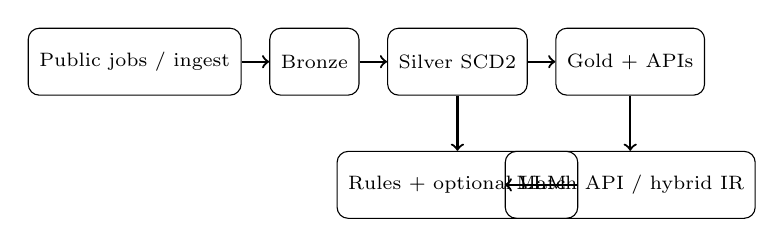
\begin{tikzpicture}[
  font=\scriptsize,
  box/.style={draw, rounded corners, align=center, inner sep=4pt, minimum height=0.85cm},
  arr/.style={->, thick}
]
\node[box] (ing) {Public jobs / ingest};
\node[box, right=0.35cm of ing] (br) {Bronze};
\node[box, right=0.35cm of br] (si) {Silver SCD2};
\node[box, right=0.35cm of si] (go) {Gold + APIs};
\node[box, below=0.7cm of si] (en) {Rules + optional LLM};
\node[box, below=0.7cm of go] (ma) {Match API / hybrid IR};
\draw[arr] (ing) -- (br);
\draw[arr] (br) -- (si);
\draw[arr] (si) -- (go);
\draw[arr] (si) -- (en);
\draw[arr] (en) -- (ma);
\draw[arr] (go) -- (ma);
\end{tikzpicture}
\caption{Extra generative layer on the existing DataForge medallion pipeline (TikZ fallback).}
\label{fig:arch}
\end{figure}

\begin{figure}[ht]
\centering
\maybeincludegraphics[width=0.92\textwidth]{figures/architecture.png}
\caption{DataForge architecture with generative integration layer (place \texttt{figures/architecture.png} or \texttt{figures/architecture.pdf} in the Overleaf project).}
\label{fig:arch-png}
\end{figure}

Public job documents still flow through Bronze and Silver. Generative components read Silver and Gold. They do not rewrite slowly changing dimension keys.

\subsection{Model gateway}

\texttt{ModelRouter} implements task types (\texttt{enrich}, \texttt{embed}, \texttt{explain}). Production order is \textbf{OpenAI first} (\texttt{gpt-4o-mini} and \texttt{text-embedding-3-small}) while Amazon Bedrock Nova Micro quota stays at zero. Bedrock in \texttt{eu-central-1} remains the preferred EU-resident path when quota is approved. OpenAI, Anthropic, and local models stay as fallbacks. The router checks JSON schema, logs cost, checks a daily budget, and uses the \texttt{AI\_ENABLED} stop switch. Prompt versions are stored under \texttt{prompts/}. Match can load vectors from LanceDB when the library is installed. It falls back to \texttt{embedding\_index.json} when the LanceDB wheel is missing in Lambda.

\subsection{Rules-first enrichment}

Fixed German/English classifiers assign tech field, seniority, visa stance, languages, and derived flags. Language-model calls happen only when they are turned on, and only when rules mark a case as unclear or a sample rate allows it. Silver and Gold schemas gain extra columns. SCD logic is not changed.

\subsection{Retrieval and Match API}

BM25, dense ranking, and reciprocal rank fusion implement hybrid retrieval. FastAPI exposes \texttt{/health}, \texttt{/jobs}, \texttt{/match}, and \texttt{/match/agent}. Production uses a Function URL with a 60-second timeout, an optional API key, CORS, and personal-data removal. An in-process graph (Supervisor $\rightarrow$ Retriever $\rightarrow$ Scorer $\rightarrow$ Explainer $\rightarrow$ Critic) is optional and limited. A Model Context Protocol server exposes \texttt{search\_jobs}, \texttt{get\_job}, and \texttt{match\_resume}.

\subsection{Operational status at measurement time}

Table~\ref{tab:status} records the status on 1 October 2026. The lakehouse, Match API, and OpenAI enrichment path are live. Bedrock completions are still blocked by a zero quota.

\begin{table}[ht]
\centering
\caption{Operational status at measurement time (1 October 2026)}
\label{tab:status}
\begin{tabularx}{\textwidth}{@{}lX@{}}
\toprule
\textbf{Capability} & \textbf{Status} \\
\midrule
Lakehouse, Jobs/Metrics APIs, Pages & Live \\
Match Function URL with API key & Live \\
Nightly OpenAI enrichment (sample rate 0.25) & Live (304 product-board jobs $\rightarrow$ 28 LLM rows) \\
LanceDB vector path & Code + Terraform; JSON index fallback in Lambda \\
Nightly Bedrock enrichment & Paused (Nova Micro quota 0; case still open) \\
RQ2 live OpenAI Pareto (\texttt{gpt-4o-mini}) & Complete (40/40) \\
RQ2 live Bedrock Pareto & Pending quota approval \\
RQ3 labelled matching evaluation & Complete (103$\times$96) \\
RQ4 modelled unit cost + live CostLogger & Complete \\
Faithfulness structural spot-check & Complete (20 citations; LLM judge optional) \\
\bottomrule
\end{tabularx}
\end{table}

\section{RQ1 --- Integration without breaking data history}
\label{sec:rq1-results}

Checks of schemas, Terraform modules (\texttt{terraform/ai.tf}), and the budget runbook show the following. Enrichment columns are extra columns. The router does not write \texttt{job\_id} or SCD validity fields. \texttt{AI\_ENABLED} and a daily budget exist. Enrichment EventBridge is on at \texttt{cron(30 21 * * ? *)} UTC with OpenAI-first sampling. Silver-to-Gold Step Functions Express is present, with the extra schedule off by default. The Bedrock quota pause stopped only the Nova Micro path. It did not require a redesign of keys. RQ1 is therefore answered at the level of architecture, code, and a live OpenAI enrichment run, with the Bedrock limit in Table~\ref{tab:status}.

\section{RQ3 --- Matching quality}
\label{sec:rq3}

Table~\ref{tab:rq3} reports ranked retrieval quality on \textbf{103} graded queries and 96 jobs (expanded from a 42-query pilot). Figure~\ref{fig:rq3-bars} visualises nDCG@10. Detail notes live in \texttt{evals/results/error\_analysis.md}.

\begin{table}[ht]
\centering
\small
\caption{Matching quality on the labelled set (RQ3; 103$\times$96)}
\label{tab:rq3}
\begin{tabular}{@{}lrrrr@{}}
\toprule
\textbf{Method} & \textbf{nDCG@10} & \textbf{P@5} & \textbf{Recall@20} & \textbf{MRR} \\
\midrule
BM25 & 0.1351 & 0.1437 & 0.1926 & 0.1906 \\
Dense & 0.2174 & 0.2175 & 0.2856 & 0.2706 \\
Hybrid & 0.1668 & 0.1670 & 0.2225 & 0.2327 \\
Heuristic wizard & 0.1462 & 0.1728 & 0.2071 & 0.1952 \\
\bottomrule
\end{tabular}
\end{table}

\begin{figure}[ht]
\centering
\maybeincludegraphics[width=0.78\textwidth]{figures/rq3_bars.png}
\caption{nDCG@10 by retrieval method on the 103-query labelled set (packaging semantic-embed run).}
\label{fig:rq3-bars}
\end{figure}

\begin{table}[ht]
\centering
\small
\caption{Matching quality under the CI local tf-idf embedding pin (103$\times$96, 1 October 2026)}
\label{tab:rq3-ci}
\begin{tabular}{@{}lrrrr@{}}
\toprule
\textbf{Method} & \textbf{nDCG@10} & \textbf{P@5} & \textbf{Recall@20} & \textbf{MRR} \\
\midrule
BM25 & 0.1351 & 0.1437 & 0.1926 & 0.1906 \\
Dense (local tf-idf) & 0.1258 & 0.1204 & 0.1869 & 0.1835 \\
Hybrid (local tf-idf) & 0.1268 & 0.1262 & 0.1885 & 0.1837 \\
Heuristic wizard & 0.1462 & 0.1728 & 0.2071 & 0.1952 \\
\bottomrule
\end{tabular}
\end{table}

Dense retrieval has the highest nDCG@10 (0.2174) in the packaging run that used a semantic embedder. The rule-based wizard scores 0.1462, and BM25 scores 0.1351. Hybrid sits between dense and the wizard on this label set (0.1668). Absolute scores stay far from 1.0. H1 is supported for dense retrieval versus the wizard on that packaging run. Hybrid does not win nDCG@10 here, but remains the product default for lexical fallback and citation workflows.

Continuous integration later pins \texttt{ModelRouter} to \textbf{local tf-idf embeddings} so the gate is offline and deterministic. Under that pin, dense nDCG@10 is 0.1258 and the wizard is 0.1462 (\texttt{evals/baselines/ndcg\_baseline.json}). Table~\ref{tab:rq3} keeps the packaging semantic-embed numbers. Table~\ref{tab:rq3-ci} reports the CI pin. The two tables are not mixed.

\subsection{Error analysis by query type}
\label{sec:error-analysis}

Per-query results in \texttt{evals/results/matching\_eval.json} and \texttt{error\_analysis.md} show three patterns on the 103-query set.

\textbf{Dense wins on semantic clusters.} About 25 queries show dense ahead of the wizard by $\geq$0.05 nDCG@10. Examples include ML stack wording, role-family matching, and mixed DE/EN skill phrases where embeddings group neighbours better than fixed 60/20/20 weights.

\textbf{Heuristic or BM25 wins on exact tokens.} About eight queries each favour the wizard or BM25. Exact product names (for example Power BI), short German keyword queries, and visa/permit boilerplate often reward lexical overlap more than dense neighbours.

\textbf{Constraint-heavy queries.} Working-student, English-OK, and visa sponsorship queries stress fields that rules treat explicitly. Dense can still rank a semantically close job that fails a hard filter. Neither method understands immigration law; both read surface text.

Table~\ref{tab:error-patterns} summarises where dense wins or fails versus the wizard.

\begin{table}[ht]
\centering
\caption{Qualitative error patterns (RQ3)}
\label{tab:error-patterns}
\begin{tabularx}{\textwidth}{@{}lXX@{}}
\toprule
\textbf{Theme} & \textbf{Dense tends to} & \textbf{Wizard tends to} \\
\midrule
Skill synonyms (PyTorch / deep learning) & Win & Miss if keywords differ \\
German/English mixed titles & Win partially & Miss without bilingual rules \\
Visa sponsorship wording & Confuse similar employers & Miss if visa not in skill tokens \\
Seniority (Intern vs Senior) & Confuse adjacent levels & Win when title tokens match \\
Empty corpus slice (q04--q09) & Fail equally & Fail equally \\
\bottomrule
\end{tabularx}
\end{table}

\subsection{German and English mixed text}

Sample jobs pair German HR phrases (``Werkstudent'', ``Flie{\ss}end Deutsch (C1)'') with English skill lists. BM25 and the wizard depend on token overlap. Dense embeddings partially bridge language if the encoder saw both languages during training. This explains part of the dense advantage on AI/ML queries. It does not remove the need for explicit language and visa rules in enrichment. Rules-first labels for \texttt{visa\_stance} and \texttt{working\_language} are meant to support filters later, not to fix retrieval alone.

\section{RQ2 --- Provider trade-offs}
\label{sec:rq2}

Table~\ref{tab:rq2} reports the live Pareto point on 1 October 2026. The runner pinned OpenAI \texttt{gpt-4o-mini} with a strict pin (no silent local fallback). Rules complete 40/40 jobs at almost zero latency and \EUR{0} model spend. OpenAI completes 40/40 jobs at about 1125\,ms average latency and \$0.0011 total cost.

\begin{table}[ht]
\centering
\caption{RQ2 live Pareto (n=40 jobs; 1 October 2026)}
\label{tab:rq2}
\begin{tabular}{@{}lrrrr@{}}
\toprule
\textbf{Path} & \textbf{n ok} & \textbf{Avg latency} & \textbf{Total USD} & \textbf{Provider} \\
\midrule
Rules only & 40/40 & 0.18 ms & 0.000 & rules \\
OpenAI \texttt{gpt-4o-mini} & 40/40 & 1125 ms & 0.0011 & openai \\
Bedrock Nova Micro & --- & --- & --- & blocked (quota 0) \\
\bottomrule
\end{tabular}
\end{table}

Amazon Nova Micro remains blocked at 0 tokens/minute and 0 tokens/day. Quota case \texttt{178955627400906} (\texttt{L-DC7FF66C}) was still open. The Bedrock runner is unchanged. RQ2 is therefore \textbf{closed for OpenAI} and \textbf{still open for Bedrock}. It would be unscientific to name Bedrock a winner or a loser on latency and euro cost.

\section{Rules enrichment quality}
\label{sec:rules-f1}

On 150 labelled jobs, rules-first classifiers reach macro-F1 of 1.0 for tech field and seniority. Visa stance macro-F1 is 0.77. The weak class is \texttt{existing\_permit\_required} (F1 0.0 on 16 support rows). Other visa classes (sponsorship, relocation, not mentioned, EU citizens only) are much stronger. This supports H2 in direction: cheap rules cover a large share of structured labels before any language-model call.

\section{Multi-agent ablation}
\label{sec:agent}

On the local provider, average citation-structure validity was 1.0 for both hybrid single-shot and multi-agent matching over 30 queries. The schema contract is enforced: every explanation includes \texttt{job\_id} and a text span pointer.

\subsection{Faithfulness spot-check}

A later hybrid citation check (\texttt{evals/run\_faithfulness\_spotcheck.py}, 1 October 2026) scored structural validity 1.0 on 20 citations from an offline fixture. An optional LLM judge was not run in that pass (\texttt{llm\_faithfulness\_rate} is empty). Structural validity still does not prove that the explanation text is true under a live completion model.

\subsection{Interpretation of the ablation}

A score of 1.0 on structural validity means the JSON shape is correct. It does not mean the explanation text is true. The local provider returns templated summaries. Both single-shot and multi-agent paths satisfy the same Pydantic schema. The multi-agent path adds latency and more moving parts. On this stub, it did not add measurable structural benefit. The ablation therefore supports \emph{keeping agents optional} until a live faithfulness test shows a gain. This matches the FrugalGPT idea: do not pay for extra steps without evidence \cf{chen2023frugalgpt}.

\section{RQ4 --- Unit cost}
\label{sec:rq4}

Table~\ref{tab:roi} reports the modelled OpenAI-first production path: 1{,}000 jobs with rules-first enrichment (about 30\,\% language-model calls), embeddings for the corpus, and 100 match requests. Public \texttt{gpt-4o-mini} and \texttt{text-embedding-3-small} list prices are used. The FX rate is 0.92.

\begin{table}[ht]
\centering
\caption{Modelled unit cost for a 1{,}000-job scenario (OpenAI-first)}
\label{tab:roi}
\begin{tabular}{@{}lrr@{}}
\toprule
\textbf{Component} & \textbf{USD} & \textbf{EUR} \\
\midrule
Enrichment, language model on full corpus & 0.330 & 0.304 \\
Enrichment, rules-first (30\,\%) & 0.099 & 0.091 \\
Embeddings (\texttt{text-embedding-3-small}) & 0.009 & 0.008 \\
Total, rules-first path & 0.108 & 0.099 \\
\bottomrule
\end{tabular}
\end{table}

Under these assumptions the rules-first OpenAI path costs about \EUR{0.10} per thousand jobs. A live CostLogger flush from the RQ2 OpenAI run (40 enrich calls) totals \$0.0011, or about \EUR{0.025} per thousand jobs as an enrich-only proxy. Nova Micro plus Titan Embed remain cheaper on the price list once Bedrock quota opens. Control tools in software include sample rate, daily budget, stop switch, Match API key, and schedule pause.

\section{Threats to validity}
\label{sec:threats}

Construct validity: nDCG@10 measures ranked relevance on labels written by the author. It does not measure hiring outcomes. Internal validity: the dense advantage may partly reflect how labels were written and which jobs exist in the 96-job slice. External validity: one lakehouse, one junior-oriented query mix, and one cloud region. Statistical conclusion validity: 103 queries are enough for an applied MSc pilot, not for a very large IR significance programme. Labels remain author-constructed. Measurement validity for RQ3: the packaging table used a semantic embedder; the CI gate pins local tf-idf and must not be mixed into Table~\ref{tab:rq3}. Conclusion validity for RQ2 is closed for OpenAI and still limited for Bedrock by the quota gap. Operational validity: quota rules are part of real MLOps; treating them as experimental conditions is honest \cf{kreuzberger2023mlops}.

\chapter{Discussion}
\label{ch:discussion}

This chapter contains my own interpretation, practical application, and critical judgement. The numbers themselves stay those of Chapter~\ref{ch:results}.

\section{Answering the research questions}
\label{sec:answers}

Table~\ref{tab:rq-answers} summarises my reading of the evidence at draft time.

\begin{table}[ht]
\centering
\caption{Author's answers to the research questions}
\label{tab:rq-answers}
\begin{tabularx}{\textwidth}{@{}lX@{}}
\toprule
\textbf{RQ} & \textbf{Answer} \\
\midrule
RQ1 & Integration without breaking SCD keys is possible. Extra schemas, identity that cannot change, Terraform isolation of AI resources, and a stop switch are enough. Nightly OpenAI enrichment is live at sample rate 0.25. A Bedrock quota pause is an operations incident. It does not prove that the architecture is wrong. \\
RQ2 & Closed for OpenAI: \texttt{gpt-4o-mini} completed 40/40 jobs at about \$0.0011 and 1.1\,s. Not closed for Bedrock: Nova Micro quota is still zero. It would be unscientific to name a Bedrock winner. \\
RQ3 & On the packaging semantic-embed run, dense retrieval beats the rule-based wizard on nDCG@10 (0.217 vs 0.146). H1 is supported for that run. Under the CI local tf-idf pin, the wizard is higher (0.146 vs 0.126). Hybrid is not the nDCG winner. It can still be a reasonable product default. \\
RQ4 & Modelled OpenAI-first spend at 1{,}000 jobs is about \EUR{0.10} when rules-first sampling is used. Live CostLogger on 40 enrich calls is cents. H2 and H4 are supported only in direction, and only under list-price plus live OpenAI assumptions. \\
\bottomrule
\end{tabularx}
\end{table}

\section{Why dense can win on the gold set while hybrid is still used}
\label{sec:dense-vs-hybrid}

A tempting conclusion is ``stop using BM25''. That conclusion would ignore both the IR literature and the product needs. Reciprocal rank fusion exists because collections and queries are mixed \cf{cormack2009rrf}. BEIR shows that the best retriever changes by domain \cf{thakur2021beir}. The Career Matching Wizard must stay explainable. Keyword hits map cleanly onto highlighted evidence spans. This matters for citations and for GDPR-style transparency \cf{eu2016gdpr,edwards2021regulating}. Hybrid retrieval is therefore not a failed experiment. It is a compromise with more than one goal. The scientific claim that is actually supported is narrower: embedding retrieval improves nDCG@10 compared with the 60/20/20 rules on this junior-oriented gold set \emph{when a semantic embedder is used}. Under the later CI local tf-idf pin, H1 is not supported. That difference is a measurement fact. It shows why the thesis must name the embedder.

The absolute scores (nDCG@10 $\approx$ 0.22 at best) come from honest labelling. They are not a defect of the methods. Scores near 1.0 on a tiny set would be easier to market and weaker as science.

\section{Reading the error analysis}
\label{sec:error-discussion}

The zero scores on queries q04--q09 are important for supervisors and for future work. They show that average nDCG is not a single story. A product demo can show one good ML query. A thesis must also show where the corpus fails. In my view, expanding the job slice for DevOps, SAP, and product roles is a data-coverage task first. It is not solved by a larger language model alone.

Visa and language constraints expose a deeper issue. Job text often states visa rules indirectly (``EU citizens only'', ``relocation support'', ``Blue Card''). Dense retrieval may treat two ML internships as similar even when only one offers sponsorship. The wizard does not solve this either unless visa tokens appear in the weighted fields. Rules-first enrichment of \texttt{visa\_stance} is the right long-term path. Retrieval and enrichment must be judged together. Chapter~\ref{ch:implications} returns to this point.

Seniority confusion (intern versus working student versus graduate) is a labelling and taxonomy problem as much as a vector problem. German employers use different words for similar levels. A single embedding space helps, but taxonomy columns in Silver still matter for filters and for fair user expectations.

\section{Quota as an experimental variable}
\label{sec:quota}

In my view, applied generative-AI theses should treat billing and quota rules as first-class experimental limits, equal to model choice. The FrugalGPT literature already treats cost as a performance dimension \cf{chen2023frugalgpt}. Account-level token caps are only a harder form of the same dimension. Reporting ``architecture complete / measurement pending'' with a fixed protocol is better than silently changing provider in the middle of the study. It is also better than inventing a Pareto table.

This incident also shows why \texttt{AI\_ENABLED} and schedule pauses are not optional extras. They are part of scientific control. When Bedrock quota returns, the same runner should fill the missing Nova Micro cells without rewriting the thesis method. Until then, production uses OpenAI-first and reports that choice openly. Switching provider in silence would be worse science than saying ``OpenAI measured; Bedrock blocked''.

\section{Practical application}
\label{sec:practical}

For platform teams that already own a medallion pipeline, the practice to copy is: freeze identity and history; add AI as a join; measure against a simple baseline; put a budget in the request path; prefer in-region inference when the product is European. For career-product owners, the practice to copy is: do not sell raw dumps of public vacancies as intelligence; sell cited shortlists, visa/entry filters, and quality-checked history. For supervisors of applied master's projects, the practice to copy is: require a non-AI baseline and a stop switch before a language-model diagram is accepted as a contribution.

Holstein et al.\ remind us that practitioners want tools that fit workflow, not only accuracy tables \cf{holstein2019improving}. DataForge Match is small, but it already follows that idea: API key, citations, and a wizard that stays available when AI is off.

\section{Responsible-AI judgement}
\label{sec:rai-discussion}

In my judgement, DataForge Match is an advice tool for job discovery. It should not be described as a high-risk employment system in the AI Act sense, because it does not rank people for an employer \cf{eu2024aiact,veale2021demystifying}. Annex~III of the AI Act lists recruitment and selection of natural persons among high-risk uses when they affect access to employment. The Match API ranks \emph{vacancies} for a user who asked for help. That is closer to a search and recommendation service than to automated rejection of candidates.

This legal reading does not remove remaining ethics duties. Visa heuristics can still harm if they are presented as certainty. A ``visa sponsorship likely'' label is not legal advice. Resume text is still personal data under the GDPR \cf{eu2016gdpr}. Citations can still have a valid structure and a wrong meaning. The human-in-the-loop queue, data removal, and ``not legal advice'' disclaimers are therefore still needed, even if the risk class is lower than employer screening.

I also reject the opposite mistake: claiming ``low risk'' and then hiding automation. Job seekers deserve to know that ranking is automated, that evidence comes from public text, and that they should verify visa and language rules with the employer. Edwards and Veale argue that meaningful information about automated decisions can be required even when a full explanation right is narrow \cf{edwards2021regulating}. UI copy and API responses are part of responsible design, not marketing.

Fairness literature warns against abstract fixes that ignore context \cf{selbst2019fairness,barocas2023fairness}. For seeker-side ranking, fairness means exposure to relevant roles across locations and language groups, not parity of false positives in hiring. This thesis cannot measure long-run exposure. It can require citations and document limits.

\section{Comparison with related work}
\label{sec:compare-lit}

Person--job fit papers often report higher metrics on academic résumé datasets \cf{qin2018personjob}. Those datasets are cleaner and larger than a 96-job pilot. Karpukhin et al.\ report strong dense retrieval on open-domain QA \cf{karpukhin2020dpr}. Job search mixes HR boilerplate and legal hints. That is closer to BEIR ``heterogeneous'' settings than to QA \cf{thakur2021beir}. The modest nDCG here is therefore not shocking. It is a reason to avoid copying QA leaderboard numbers into product slides.

\section{Limitations}
\label{sec:limitations}

The labelled set is small. The annotator and the system author are the same person. RQ2 live Bedrock cells are missing. Multi-agent semantic faithfulness under a live completion model is still untested (only structural checks ran). Coverage of German vacancies is still incomplete. Visa stance is often \texttt{not\_mentioned} in the raw text. This limits product KPIs even when the model is good. Official binding details (matriculation number, signed supervisors, Examination Office declaration if it differs) were not all available at draft time.

\section{Comparison of the expanded label set with the pilot}
\label{sec:label-scale}

The first pilot used 42 queries. The expanded set uses 103 queries on the same 96-job corpus. Mean nDCG@10 for dense retrieval moved only slightly (from about 0.220 to 0.217). The wizard and BM25 scores also stayed in the same band. This stability is useful. It suggests that the dense advantage is not an artefact of a tiny query list alone. Absolute scores remain modest. That is expected for a synthetic but graded corpus that mixes languages, visa phrases, and seniority words. Future work should add a second human annotator and more real vacancy text from Gold, not only more synthetic queries.


\chapter{Implications and Future Research}
\label{ch:implications}

\section{Theoretical implications}
\label{sec:theory-impl}

Three implications follow for the scientific discussion in Chapters~\ref{ch:theory-data} and~\ref{ch:theory-ai}.

First, lakehouse research should treat generative models as a new class of extra data user, in Sculley's sense, unless layer contracts name them clearly \cf{sculley2015debt,armbrust2021lakehouse}. The contribution of this case is to show that dimensional history and embeddings can exist together if identity is frozen.

Second, IR evaluation remains the correct language for ``AI matching'' claims. nDCG, a keyword baseline, and a gold set that is not almost perfect stop augmented-analytics talk from becoming only a demo \cf{jarvelin2002ndcg,manning2008ir}. Dense retrieval's advantage here is consistent with Karpukhin et al.\ on other collections. However, the modest absolute scores warn against copying open-domain question-answering numbers into job search \cf{karpukhin2020dpr,thakur2021beir}.

Third, design science is a sufficient, and for an applied M.Sc.\ an honest, frame. The knowledge produced is a working system with measured properties. It is not a new law of retrieval. Hevner requires that artefacts are evaluated with methods that match the claims. Gregor and Hevner add that the contribution must be positioned so reviewers see design and evaluation together \cf{hevner2004dsr,gregor2013positioning}. This demand is met only if RQ2's missing \emph{Bedrock} cells are disclosed, and if the OpenAI live cells are reported as OpenAI, not as in-region Bedrock.

\section{Practical and managerial implications}
\label{sec:practical-impl}

For European product organisations the case suggests an order: data contracts, then rules, then embeddings, then generation, then agents. Turning this order around increases spend and reduces auditability. Hyperautomation slogans that skip the first two steps are, on this evidence, weak in operations \cf{gartner2020hyper}.

Unit cost at OpenAI \texttt{gpt-4o-mini} prices is still cents at 1{,}000-job scale (about \EUR{0.10} modelled). Nova-class prices would be lower still. The scarce resources are labelled evaluation, quota control, and trust, not token spend at this size. Monetisation should therefore attach to cited Match, quality-checked history, and location guarantees, not to CSV dumps of public jobs.

For public employment data specifically, advisory matching can reduce search cost for juniors without becoming an automated hiring gate. That product boundary should be written into terms of service and into colloquium slides, not only into a legal appendix. Practitioners should train support staff to explain the difference between \emph{job ranking for seekers} and \emph{candidate ranking for employers}. Veale and Borgesius show that AI Act categories depend on intended purpose \cf{veale2021demystifying}. Product copy is part of compliance work.

Raji et al.\ suggest internal auditing before launch \cf{raji2020closing}. Even a student project can adopt a light version: log prompts, log costs, keep evaluation files in git, and document pauses. That habit transfers directly to industry MLOps \cf{kreuzberger2023mlops}.

\section{Implications for job seekers and career services}
\label{sec:seeker-impl}

From a seeker perspective, the useful output is not a single score. It is a short list with reasons: matched skills, location, seniority fit, and a visa hint with citation. Users who need English-only roles or sponsorship benefit when language and visa columns are explicit in Gold, not only when embeddings guess similarity. Users who search in German benefit when rules normalise ``Werkstudent'' and ``working student'' to the same seniority band.

Career centres at universities could reuse the Match API as a teaching tool. Students see how the same resume changes rank order under BM25, dense, and hybrid methods. That builds literacy about automated job search without pretending the system is neutral or complete.

\section{Implications for the University of Europe Data Science profile}
\label{sec:ue-impl}

The programme asks students to connect data engineering, statistical evaluation, and responsible application. A thesis that only deploys a vendor chatbot would fail that profile. A thesis that only reviews literature would fail the built-system expectation of an applied degree. The implication for future UE theses in this area is practical: register a title that names the \emph{integration problem}, freeze an evaluation protocol before the writing clock starts, and keep a measurement log that can survive a quota incident.

The literature share expected for a 120 ECTS master's thesis is large. This project meets that expectation by giving two theory chapters, not a short related-work paragraph. Sources are graded in Appendix~\ref{app:sources}. Page-level Harvard citations should still be added after final reading of each monograph.

\section{Future research}
\label{sec:future}

Several extensions are possible in a short time after submission, or in a follow-on paper (optional IEEE 4--8 pages, as offered in the colloquium).

\begin{enumerate}
  \item Complete the RQ2 live Bedrock Pareto table after Nova Micro quota approval, without changing the runner. OpenAI cells are already filled.
  \item Add a second annotator on the 103-query gold set, and report agreement between annotators.
  \item Add job slices for q04--q09 themes so coverage gaps can be retested.
  \item Run the optional LLM faithfulness judge on hybrid citations, not only structural validity.
  \item Compare in-region Bedrock embeddings with OpenAI \texttt{text-embedding-3-small} and an open encoder on the same jobs.
  \item Run a small user study with intern and working-student seekers (ethics approval, informed consent) to add preference judgements next to nDCG.
  \item Test whether rules-first cleaning of seniority and visa fields improves dense retrieval. This links the colloquium topic of automated data cleaning to ranking quality.
  \item Explore continuous experimentation in production with a careful traffic split after faithfulness checks pass \cf{fagerholm2017right}.
\end{enumerate}

Topics that are not recommended as immediate extensions are quantum ranking, unsupervised module clustering of the code base, and automated fault finding. They are real software-engineering agendas from the colloquium list. However, they would replace the research questions rather than deepen them.

\section{Conclusion}
\label{sec:conclusion}

This thesis asked how generative AI can be added to a live European job-intelligence lakehouse without destroying history, evaluation honesty, or a free-tier budget. The literature placed the problem at the meeting point of digitalisation, dimensional modelling, information retrieval, LLM operations, and European law. Design science with one embedded case was chosen over a literature-only or survey design because the questions are about a system under limits.

On labelled matching data, dense retrieval improved nDCG@10 compared with a clear rule-based wizard in the packaging semantic-embed run. Hybrid retrieval did not win that table. It still remains the product default for keyword robustness and citation workflows. Modelled OpenAI-first enrichment and embedding costs at 1{,}000 jobs stay around ten euro cents when rules-first sampling is used. Live OpenAI RQ2 is complete (40/40). Live Bedrock completion experiments remain open, pending a cloud quota. Those sentences are the empirical core. Everything else is architecture, law, and caution.

The work shows that an M.Sc.\ Data Science thesis at the University of Europe can be both a production portfolio and a testable integration study. This is possible if generative AI is treated as a controlled pipeline stage, not as slideware.

\section{What this thesis does not claim}
\label{sec:nonclaims}

This thesis does not claim that dense retrieval solves visa uncertainty. It does not claim that Bedrock is cheaper than OpenAI on this account; the live Bedrock Pareto cells are still pending. It does not claim that the Match API is a hiring system. It does not claim that 103 author-labelled queries equal an industry benchmark such as BEIR. It does not mix the CI local tf-idf nDCG with the packaging semantic-embed table. Clearing these non-claims keeps the contribution testable and aligned with the writing lecture's demand for a thesis, not an essay.



% -------------------------------------------------------------------------
% Bibliography (Harvard / author-year)
% -------------------------------------------------------------------------
\clearpage
\bibliographystyle{apalike}
\bibliography{references}
\addcontentsline{toc}{chapter}{Bibliography}

% -------------------------------------------------------------------------
% Appendices
% -------------------------------------------------------------------------
\appendix
\chapter{Artefact map}
\label{app:artefacts}

\begin{table}[ht]
\centering
\caption{Primary thesis artefacts in the repository}
\label{tab:artefacts}
\begin{tabularx}{\textwidth}{@{}lX@{}}
\toprule
\textbf{Artefact} & \textbf{Path} \\
\midrule
Expos\'e for supervisors & \texttt{docs/thesis/THESIS\_EXPOSE.md} \\
Registration-style proposal & \texttt{docs/thesis/THESIS\_PROPOSAL.md} \\
UE requirements note & \texttt{docs/thesis/UE\_REQUIREMENTS.md} \\
Results ledger & \texttt{docs/thesis/RESULTS\_DRAFT.md} (if present) \\
This \LaTeX{} project & \texttt{docs/thesis/latex/} \\
Matching evaluation & \texttt{evals/results/eval\_report.md} \\
Matching JSON & \texttt{evals/results/matching\_eval.json} \\
Error analysis & \texttt{evals/results/error\_analysis.md} \\
RQ2 Pareto JSON & \texttt{evals/results/rq2\_pareto.json} \\
ROI model & \texttt{evals/results/roi\_report.json} \\
Agent ablation & \texttt{evals/results/agent\_ablation.json} \\
Faithfulness spot-check & \texttt{evals/results/faithfulness\_spotcheck.json} \\
Colloquium outline & \texttt{docs/thesis/COLLOQUIUM\_OUTLINE.md} \\
Demo script & \texttt{docs/DEMO\_SCRIPT.md} \\
Technical guide (plain English) & \texttt{docs/TECHNICAL\_GUIDE\_EASY\_ENGLISH.md} \\
Terraform AI module & \texttt{terraform/ai.tf} \\
Match API & \texttt{services/match/} (repository layout) \\
Figure placeholders & \texttt{docs/thesis/latex/figures/architecture.png}, \texttt{rq3\_bars.png} \\
\bottomrule
\end{tabularx}
\end{table}

\chapter{Reproduction commands}
\label{app:repro}

All commands assume the repository root \texttt{d:\textbackslash dataforge} (or the cloned GitHub path). Python 3.10+ is required. Install project dependencies from \texttt{requirements.txt} or the service-specific file before running evals.

\begin{lstlisting}[language=bash,caption={Reproduction commands for the empirical tables}]
# Matching evaluation (RQ3) -> evals/results/matching_eval.json
py -3 evals/run_matching_eval.py

# Rules enrichment evaluation
py -3 evals/run_enrichment_rules_eval.py

# Agent ablation (structural citation validity)
py -3 evals/run_agent_ablation.py

# ROI model (RQ4) -> evals/results/roi_report.json
py -3 scripts/roi_report.py

# Faithfulness structural spot-check
py -3 evals/run_faithfulness_spotcheck.py --limit 20

# RQ2 live OpenAI (current production pin)
set AI_ENABLED=true
py -3 evals/run_rq2_pareto.py --live-providers --provider openai --strict-pin --limit 40

# RQ2 live Bedrock (after Nova Micro quota approval)
set AWS_PROFILE=dataforge-germany
set BEDROCK_COMPLETION_MODEL=eu.amazon.nova-micro-v1:0
py -3 evals/run_rq2_pareto.py --live-providers --provider bedrock --limit 40

# Compile thesis (Overleaf: set main document to overleaf_main.tex)
# Local: pdflatex + bibtex in docs/thesis/latex/
\end{lstlisting}

Measured outputs should be committed or archived with a date stamp. If RQ3 numbers change after corpus expansion, update Table~\ref{tab:rq3} and note the change in Appendix~\ref{app:changelog}.

\chapter{Administrative note for binding}
\label{app:admin}

Before binding, the student must fill in Overleaf macros in \texttt{overleaf\_main.tex}:

\begin{itemize}
  \item \texttt{\textbackslash Matrikel\{\}} --- matriculation number;
  \item \texttt{\textbackslash Erstbetreuung\{\}} and \texttt{\textbackslash Zweitbetreuung\{\}} --- supervisor names;
  \item \texttt{\textbackslash Abgabedatum\{\}} --- submission date.
\end{itemize}

Replace the statutory declaration page if the Pr\"ufungsamt publishes different official wording. Add access dates to internet sources (BA/EURES documentation) in the bibliography notes. Replace preprint entries (FrugalGPT, foundation-model report, RAG survey) with published versions if they appear before submission.

The University of Europe 120 ECTS master's thesis target is roughly 72{,}000--82{,}000 characters \emph{without spaces} in the body. Use the word processor or a script to count before binding. AI-assisted drafting must be rewritten in the student's own voice; AI detection above 20\,\% is a fail condition per programme guidance.

\chapter{Source hierarchy used in the literature review}
\label{app:sources}

The University of Europe asks students to describe the quality of cited sources. Table~\ref{tab:hierarchy} groups the bibliography.

\begin{table}[ht]
\centering
\caption{Hierarchy of sources (highest first)}
\label{tab:hierarchy}
\begin{tabularx}{\textwidth}{@{}lX@{}}
\toprule
\textbf{Tier} & \textbf{Examples in this thesis} \\
\midrule
Peer-reviewed journals & MIS Quarterly; ACM TOIS; JMIS; IEEE Access; JSIS; Big Data \& Society; Nature Machine Intelligence \\
IEEE / ACM / Springer / Elsevier / Sage venues & SIGIR; EMNLP; NeurIPS; ICLR; HICSS; KDD; CIDR; CHI; FAccT \\
Research monographs & Kimball and Ross (Wiley); Manning et al.\ (CUP); Yin (Sage); Bass et al.\ (Addison-Wesley); Barocas et al.\ (MIT Press) \\
Official legal texts & GDPR (EU 2016); AI Act (EU 2024) \\
Practitioner / internet (used sparingly) & Databricks medallion note; Gartner hyperautomation commentary; BA/EURES documentation \\
\bottomrule
\end{tabularx}
\end{table}

Page numbers for Harvard paraphrases should be inserted after the bound-version reading of each monograph and journal article. Preprints (FrugalGPT, foundation-model report, RAG survey) must be replaced by the archival version if one appears before submission.

\chapter{Draft change log}
\label{app:changelog}

\begin{table}[ht]
\centering
\caption{Draft change log}
\label{tab:changelog}
\begin{tabularx}{\textwidth}{@{}lX@{}}
\toprule
\textbf{Date} & \textbf{Change} \\
\midrule
16 September 2026 & Initial paper draft from proposal and measured evaluations; RQ2 marked pending quota \\
18 September 2026 & Restructured to University of Europe lecture format (Kouatly SS 2026) \\
18 September 2026 & Body text rewritten in clear academic English (IELTS Band 6 style) \\
18 September 2026 & Expanded literature (Chapters~2--2b), DSR methodology defence, RQ3 error analysis, figures placeholders, 18 new bibliography entries \\
1 October 2026 & Updated measured results: live OpenAI RQ2 40/40; OpenAI-first production and nightly enrichment; RQ4 $\approx$ \EUR{0.10}/1k; CI local tf-idf nDCG reported next to packaging table 0.2174; faithfulness structural spot-check \\
\bottomrule
\end{tabularx}
\end{table}


\end{document}
